%%%%%%%%%%%%%%%%%%%%%%%%%%%%%%%%%%%%%%%%%%%%%%%%%%%%%%%%%%%%%%%%%%%%%%%%%%

% abnTeX2: Modelo de Trabalho Acadêmico em conformidade com
% as normas da ABNT

%%%%%%%%%%%%%%%%%%%%%%%%%%%%%%%%%%%%%%%%%%%%%%%%%%%%%%%%%%%%%%%%%%%%%%%%%%

\documentclass[english,
               brazil,
               bsc] %Opções bsc (TCC) e msc (Mestrado)
               {dcomp-abntex2}


%%%%%%%%%%%%%%%%%%%%%%%%%%%%%%%%%%%%%%%%%%%%%%%%%%%%%%%%%%%%%%%%%%%%%%%%%%
% Área para adição de pacotes extras
%%%%%%%%%%%%%%%%%%%%%%%%%%%%%%%%%%%%%%%%%%%%%%%%%%%%%%%%%%%%%%%%%%%%%%%%%%

% \usepackage{lipsum} %Retirar para a versão final do documento

%Utilize aqui seu pacote preferido para algoritmos
\usepackage[linesnumbered]{algorithm2e}

%%%%%%%%%%%%%%%%%%%%%%%%%%%%%%%%%%%%%%%%%%%%%%%%%%%%%%%%%%%%%%%%%%%%%%%%%%

%Compila o indice
\makeindex

\begin{document}

% Seleciona o idioma do documento (conforme pacotes do babel)
\selectlanguage{brazil}

% Retira espaço extra obsoleto entre as frases.
\frenchspacing

%%%%%%%%%%%%%%%%%%%%%%%%%%%%%%%%%%%%%%%%%%%%%%%%%%%%%%%%%%%%%%%%%%%%%%%%%%
% ELEMENTOS PRÉ-TEXTUAIS
%%%%%%%%%%%%%%%%%%%%%%%%%%%%%%%%%%%%%%%%%%%%%%%%%%%%%%%%%%%%%%%%%%%%%%%%%%

\pretextual

\titulo{AtalaIA: Compressão de modelos de detecção facial para dispositivos embarcados de baixo custo}
\autor{Luan Fabrício de Carvalho Lima Leite}
\orientador{Leonardo Nogueira Matos}
\coorientador{Rafael Andrade da Silva}
\curso{Ciência da Computação}

\inserirInformacoesPDF

\imprimircapa
\imprimirfolhaderosto*

\begin{dedicatoria}
   \vspace*{\fill}
   \centering
   \noindent
   \textit{Dedico este trabalho a minha família, amigos, professores e todos que de alguma forma me ajudaram a chegar até aqui.}
   \vspace*{\fill}
\end{dedicatoria}
% ---

\include{Pre_Textual/Agradecimentos}
\include{Pre_Textual/Epigrafe}
% resumo em português
\setlength{\absparsep}{18pt} % ajusta o espaçamento dos parágrafos do resumo
\begin{resumo}

Redes Neurais Convolucionais estão ficando cada vez mais populares para solução de diversos desafios, sendo um deles
o de reconhecimento facial, que é uma das tarefas onde essa abordagem já supera o ser humano.
Entretanto, esse método costuma exigir um alto poder de processamento e quantidade de memória, o que acaba
limitando o seu uso em casos de computação de borda com dispositivos embarcados.
Este trabalho tem como foco tratar esse problema, comprimindo um modelo de reconhecimento facial para que ele seja
embarcado e consiga realizar operações na borda, mantendo a acurácia alta e tempo de resposta baixo.
Para que esse objetivo seja cumprido, será necessário utilizar um modelo como base, para que ele seja comprimido e
avaliado, onde ele será escolhido a partir da comparação de soluções já existentes e utilizadas.
O modelo embarcado será avaliado com base em métricas como acurácia, F1 score, latência e ocupação de memória e
comparado a outras soluções existentes.

 \textbf{Palavras-chave}: CNN, Compressão de modelos, Visão computacional, Sistemas embarcados, Computação em borda,
 Reconhecimento facial
\end{resumo}

% resumo em inglês
\setlength{\absparsep}{18pt} % ajusta o espaçamento dos parágrafos do resumo
\begin{resumo}[Abstract]
 \begin{otherlanguage*}{english}
   Convolutional Neural Networks are becoming increasingly popular for solving various challenges, one of them being
   facial recognition, which is one of the tasks that this approach overcomes humans.
   However, this method usually requires a high computational power and amount of memory, which ends up limiting its
   use case in edge computing for embedded devices.
   This work focuses on addressing this issue, compressing a facial recognition model so that it is embedded and can
   perform operations at the edge, maintaining high accuracy and low response time.
   For this objective to be achieved, it will be necessary to use a model as a basis, so that it can be compressed and
   evaluated, where it will be chosen based on the comparison of the existing and used
   solutions.
   % TODO: traduzir essa parte
   To finish, this model will be embedded to perform operations on edge, both inference and processing on the device,
   from there, its effectiveness will be measured and compared with other solutions already created.

   \vspace{\onelineskip}

   \noindent
   \textbf{Keywords}: CNN. Model compression. Computer Vision. Embedded systems. Edge computing. Facial recognition.
 \end{otherlanguage*}
\end{resumo}



\mostrarlistadeILUSTRACOES
\mostrarlistadeQUADROS
\mostrarlistadeTABELAS
\mostrarlistadeCODIGOS
\mostrarlistadeALGORITMOS

% Lista de abreviaturas e siglas

\begin{siglas}
	\item[ABNT]{Associação Brasileira de Normas Técnicas}
	\item[abnTeX]{ABsurdas Normas para TeX}
  	\item[DCOMP]{Departamento de Computação}
	\item[UFS]{Universidade Federal de Sergipe}
	\item[ANN]{Rede Neural Artificial ou \textit{Artificial Neural network}}
	\item[CNN]{Rede Neural Convolucional ou \textit{Convolutional Neural Network}}
	\item[MB]{Megabytes}
\end{siglas}

\include{Pre_Textual/Simbolos}

\mostrarSUMARIO

%%%%%%%%%%%%%%%%%%%%%%%%%%%%%%%%%%%%%%%%%%%%%%%%%%%%%%%%%%%%%%%%%%%%%%%%%%
% ELEMENTOS TEXTUAIS
%%%%%%%%%%%%%%%%%%%%%%%%%%%%%%%%%%%%%%%%%%%%%%%%%%%%%%%%%%%%%%%%%%%%%%%%%%

\textual
\chapter{Introdução}

Redes Neurais Artificiais são ferramentas poderosas para auxiliar a sociedade.
Podendo ser utilizadas em diversas tarefas, como reconhecimento facial, onde a rede é treinada para realizar a
classificação da face da pessoa, de acordo com o seu conjunto de dados.
Permitindo que ela seja usada em várias áreas diferentes, indo de entreterimento até segurança.


\section{Motivação}
O uso de Redes Neurais Artificiais vem crescendo bastante no ramo de computação visual, principalmente desde 2012,
quando Redes Neurais Convolucionais começaram a ser utilizadas para classificação de imagens \cite{alexnet}.
Um dos principais usos desse tipo de rede é na detecção de face, que é muito relevante para a área de segurança e
vigilância, onde o modelo pode fazer a detecção do rosto de uma pessoa liberar uma porta ou enviar uma notificação
para algum segurança. Porém, essa abordagem necessita de uma quantidade elevada de poder computacional, tornando
inviável que tal tipo de produto tenha um baixo tempo de resposta, o que pode atrapalhar a experiência do usuário, ou
demora muito para notificar caso alguma ação suspeita aconteça.

Um dos principais problemas das Redes Neurais é que elas necessitam de um alto processamento e uso de memória, o que
acaba dificultando a sua execução em dispositivos com poder computacional e memória limitados (como os dispositivos
embarcados).
Porém, existem técnicas que podem ser aplicadas para reduzir pode computacional necessário, como o uso de destilamento
de conhecimento \cite{hinton2015distilling}, poda e quantização.
Possibilitando a implantação do modelo em sistemas embarcados na borda, de forma que o tempo de resposta do dispositivo
seja baixo.

\section{Objetivo principal}

O objetivo deste trabalho é desenvolver uma Rede Neural Convolucional que consiga realizar a tarefa de reconhecimento
facial em dispositivos embarcados, na borda.
Para ele seja alcançado, será necessário comprimir um modelo base, para que ele necessite de pouco poder computacional
e uso de memória.

\section{Metodologia}
Para atingir o objetivo do estudo, foi necessário dividir o processo em algumas etapas, cada uma sendo
essencial para que o objetivo do trabalho seja atingido. Sendo elas:

\begin{enumerate}
	\item \textbf{Seleção de artigos:}

		Nessa etapa, são selecionados artigos que possuem o objetivo parecido com o deste artigo,
		com base nesses artigos serão testadas novas técnicas para compressão de modelos.

	\item \textbf{Seleção de base e treino de modelos:}

		Nesta é selecionada uma base de dados e a partir dela serão desenvolvidos modelos,
		com o objetivo de atingir uma alta acurácia, sem sofrer \textit{overfitting}.

	\item \textbf{Aplicação de técnicas de compressão para Modelos:}

		Após definir e treinar os modelos, serão aplicadas técnicas de compressão, tendo como
		objetivo ter uma acurácia parecida com a do modelo original. Onde as técnicas aplicadas
		foram: poda, quantização e destilamento de conhecimento.

	\item \textbf{Avaliação do desempenho:}

		Depois de treinar e aplicar técnicas de compressão, os dados dos modelos serão coletados e
		avaliados. Para realizar essa avaliação, será necessário utilizar um conjunto de teste.

	\item \textbf{Análise e comparação dos resultados:}

		Para finalizar, os dados dos modelos serão comparados e analisados. Com o objetivo de
		identificar o melhor modelo e descobrir quais foram os motivos para que esse modelo tenha se
		saído tão bem, mesmo após a aplicação de compressão. Nesta etapa as métricas de acurácia e
		tamanho do modelo são avaliadas.

\end{enumerate}

\section{Estrutura do documento}
Este documento foi divido em capítulos, onde cada um apresenta uma proposta diferente:
\begin{itemize}
	\item Capitulo 2 - \textbf{Conceitos Básicos}: Apresenta os tópicos principais para o entendimento
		do trabalho.
	\item Capítulo 3 - \textbf{Trabalhos Relacionados}: Apresenta uma revisão dos trabalhos
		relacionados ao tema do trabalho.
	\item Capítulo 4 - \textbf{Resultados Preliminares}: Apresenta os resultados preliminares dos
		experimentos realizados durante o trabalho.
	\item Capítulo 5 - \textbf{Planos de continuidade}: Contém o planejamento da continuidade do
		Trabalho de Conclusão 2.
\end{itemize}

\chapter{Conceitos básicos}\label{cap_conceitos}

\chapterprecis{
	O foco deste capítulo é introduzir alguns tópicos relevantes para o trabalho, de forma que o leitor consiga
	entender o conteúdo independente de conhecimento prévio.
	Neste capítulo serão abordados os tópicos relacionados a ANNs (\autoref{cap_conceitos_ann}),
	CNNs (\autoref{cap_conceitos_cnn}), \textit{Data augmentation} (\autoref{cap_conceitos_data_augmentation}),
	transferência de conhecimento (\autoref{cap_conceitos_transferencia}), técnicas de compressão para redes neurais
	(\autoref{cap_conceitos_compressao_redes}) e otimização Bayesiana (\autoref{cap_conceitos_bayesiana}).
}
% \chapterprecis{Isto é uma sinopse de capítulo. A ABNT não traz nenhuma
% normatização a respeito desse tipo de resumo, que é mais comum em romances
% e livros técnicos.}\index{sinopse de capítulo}

\section{Redes Neurais Artificiais}\label{cap_conceitos_ann}
% ---
Redes Neurais Artificiais (ANNs), são neurônios interconectados que realizam um processamento simples. Dentro dessa
estrutura cada neurônio reforça ou enfraquece a conexão com um dos neurônio da coluna anterior, assim replicando
o processo de aprendizagem do cérebro humano. A \autoref{cap_conceitos_ann_exemplo_ann} exemplifica uma ANN bem
simples.

\begin{figure}[htb]
	\caption {\label{cap_conceitos_ann_exemplo_ann}Exemplo de uma ANN}
	\begin{center}
		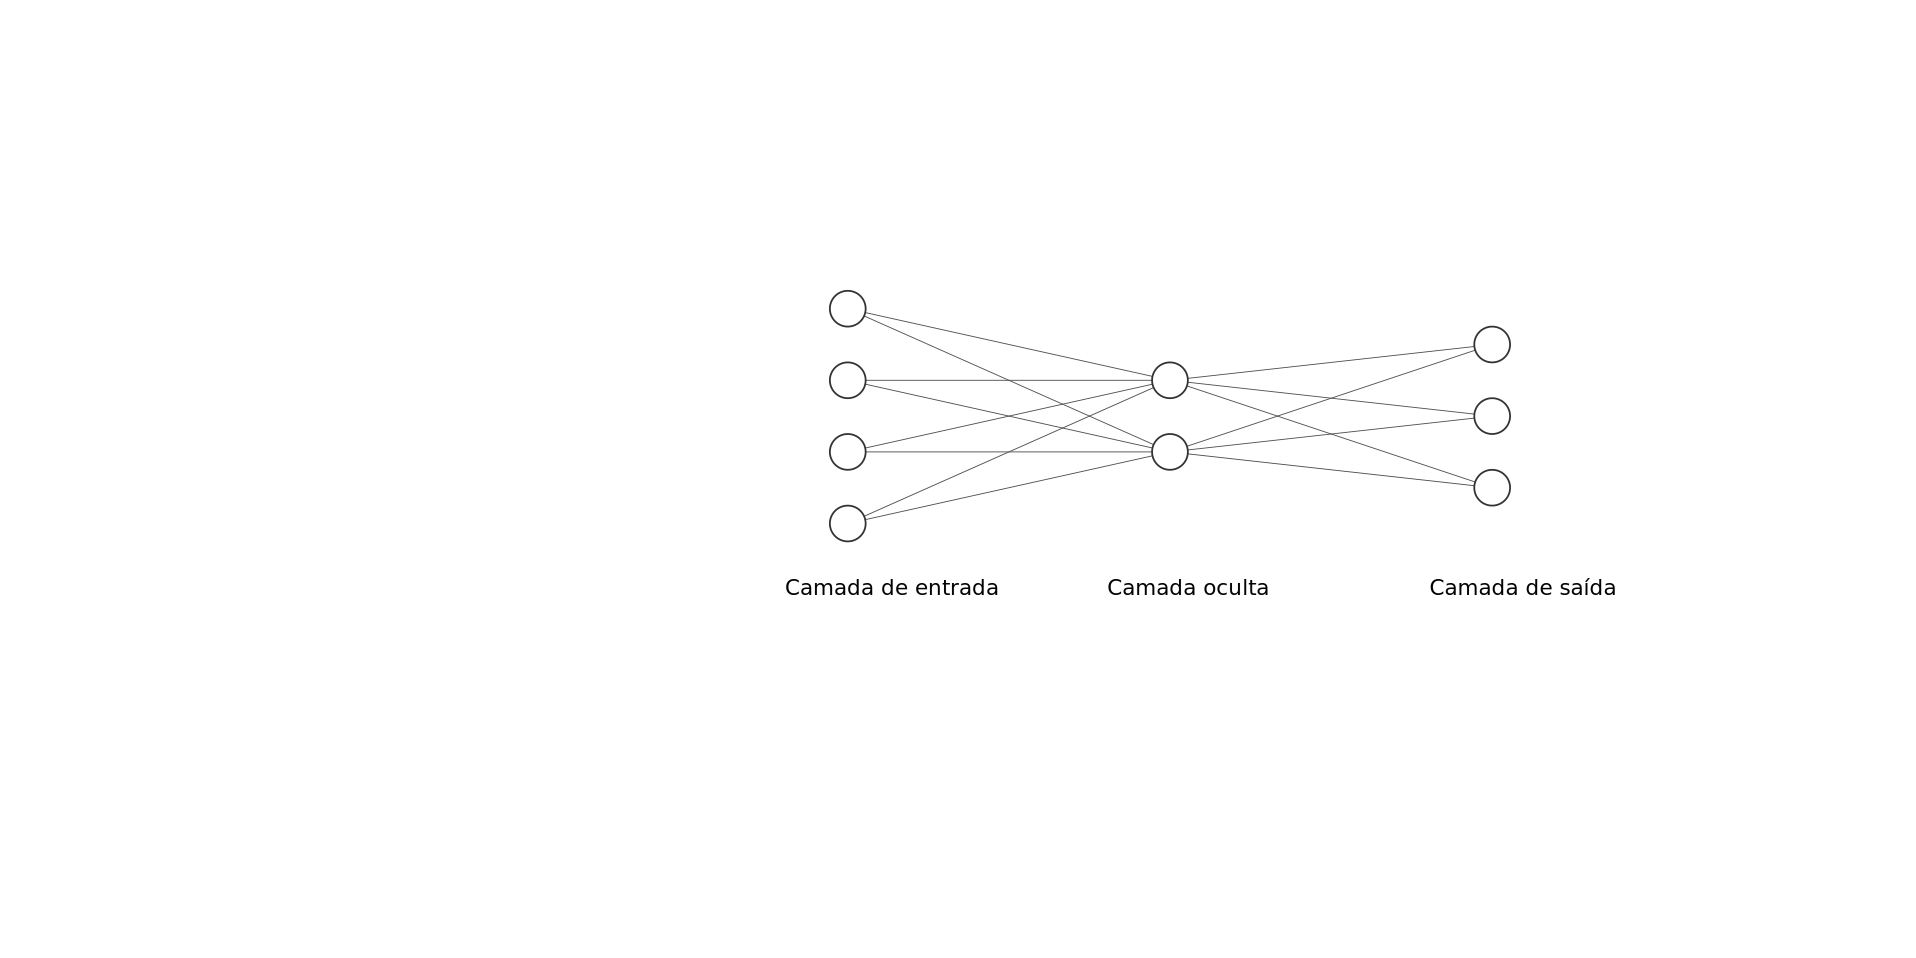
\includegraphics[scale=0.5]{Imagens/exemplo_nn}
	\end{center}
	\legend {Fonte: Autor}
\end{figure}

O neurônio é uma parte fundamental de uma ANN, nele que o aprendizado é armazenado através do reforço de conexões com
outros neurônios. Esse reforço é o peso da conexão, ele é multiplicado pela entrada e somado com os outros valores,
como é demonstrado na equação \ref{eq_neuronio} (onde $x$ é um vetor com os valores de entrada do neurônio e $w$
é um vetor com os pesos de cada entrada). Depois disso os valores passam por uma função de ativação $g(x)$ (\ref
{eq_ativacao}), que é responsável por "tratar" esses dados de saída antes que eles sejam passados para próxima etapa.

\begin{equation}\label{eq_neuronio}
u = \sum x_i w_i
\end{equation}
\begin{equation}\label{eq_ativacao}
y = g(u + b)
\end{equation}

\begin{figure}[htb]
	\caption {\label{cap_conceitos_ex_neuronio} Exemplo de um neurônio artificial}
	\begin{center}
		\includegraphics[scale=0.3]{Imagens/exemplo_neuronio_artificial}
	\end{center}
	\legend{Fonte: \cite{ml-faceli}}
\end{figure}

\section{Redes Neurais Convolucionais}\label{cap_conceitos_cnn}
% ---
Redes Neurais Convolucionais (CNNs) são Redes Neurais Artificiais (ANN)
que utilizam a operação de convolução para o processamento e análise de dados no formato de \textit{grid}(grade).
Por exemplo, uma série temporal que pode ser representada no formato de \textit{grid} 1-D,
ou uma imagem, que pode ser representada no formato 2-D. \cite{Goodfellow-et-al-2016}
Onde, LeNet \cite{lenet}, Residual Network (ResNet) \cite{resnet} e AlexNet \cite{alexnet} são alguns exemplos de CNNs
famosas.

A arquitetura de uma CNN é composta por camadas convolucionais (\ref{cap_conceitos_cnn_conv}),
\textit{pooling} (\ref{cap_conceitos_cnn_pooling}) e totalmente conectadas (\ref{cap_conceitos_cnn_totalmente}),
como podemos ver na \autoref{exemplo_lenet}.

\begin{figure}[htb]
	\caption {\label{exemplo_lenet} Arquitetura da LeNet}
	\begin{center}
		\includegraphics[scale=0.5]{Imagens/lenet}
	\end{center}
	\legend{Fonte: \cite{zhang2023dive}}
\end{figure}

\subsection{Camada de Convolução}\label{cap_conceitos_cnn_conv}
Nessa camada são aplicados filtros (matriz de pesos) nos dados de entrada,
onde esses filtros deslizam cada célula da imagem executando operações de multiplicação e soma
em cada elemento da matriz de entrada, com o objetivo de gerar um mapa de características (\textit{feature map}).
O objetivo desses filtros é realçar as características dos dados de entrada, como curvas, linhas e outros padrões.
% TODO: Adicionar figuras, referências e detalhar mais

\subsection{Camada de \textit{pooling}}\label{cap_conceitos_cnn_pooling}
% ---
A abordagem da camada de \textit{pooling} é um pouco parecida com a camada de convolução,
uma matriz desliza pelas células da imagem, salvando apenas um dos valores dessa área na matriz de saída.
A partir disso, a camada consegue reduzir o tamanho da matriz de entrada, fazendo com que o poder computacional
necessário seja reduzido, junto com o uso de memória.

Existem diversos tipos de \textit{pooling}, min, \textit{average} e max, onde cada um foca em extrair um valor dos
dados de entrada na matriz. O tipo mais comum de \textit{pooling} é o max, que salva apenas o maior valor da área,
além de reduzir o tamanho da matriz de entrada ele consegue realçar algumas características mais expressivas da matriz.
% TODO: Adicionar figuras, referências e detalhar mais

\subsection{Camada totalmente conectada}\label{cap_conceitos_cnn_totalmente}
% ---
A camada totalmente conectada (\textit{fully connected layer}) é a camada final de uma CNN.
Depois das camadas anteriores extraírem as características da imagem, ela é responsável por
fazer aprender a interpretar essas características e inferir um resultado a partir do seu treinamento.
Onde essa camada é uma ANN (\autoref{cap_conceitos_ann}) que geralmente é focada em realizar a classificação dos dados
de entrada.

\section{\textit{Data augmentation}}\label{cap_conceitos_data_augmentation}
% ---
CNNs tem um ótimo desempenho em tarefas de visão computacional. Entretanto esse tipo de rede neural precisa de uma
grande quantidade dados para não sofrer de \textit{overfitting} (superajuste). \cite{shorten2019survey}
Esse é o objetivo do \textit{data augmentation} (aumento de dados), gerar mais dados a partir de um conjunto de dados
que já existe, aplicando algumas transformações geométricas ou espaciais, ou realizando injeção de ruído nas imagens
originais.

Na \autoref{cap_conceitos_exemplo_da}, temos um exemplo de uma imagem que sofreu uma transformação para efetuar um \textit{data augmentation}.
Nesse caso, temos uma que foi flipada, gerando um novo dado para o \text{dataset}

\begin{figure}[htb]
	\caption {\label{cap_conceitos_exemplo_da}Exemplo de uma transformação utilizando \textit{data augmentation}}
	\begin{center}
		\includegraphics[scale=1]{Imagens/exemplo_da}
	\end{center}
	\legend {Fonte: \cite{tf2guia}}
\end{figure}

\section{Transferência de conhecimento}\label{cap_conceitos_transferencia}
% ---
Transferência de conhecimento consiste em usar um modelo pré-treinado em uma base de dados específica e aproveitar
o conhecimento adquirido durante esse treinamento para um novo conjunto de dados.
É necessário que o problema do \textit{dataset} (conjunto de dados) atual seja um subconjunto do \textit{dataset}
que foi usado para treinar o modelo base.

Para realizar a transferência de conhecimento é necessário adaptar a camada de entrada e de saída
(totalmente conectada) do modelo base, para que ocorra um pré-processamento dos dados de entrada
(antes deles serem passados para o modelo base), além disso é necessário definir e treinar a camada totalmente
conectada com o \textit{dataset} do problema.

\section{Métodos de compressão para Redes Neurais}\label{cap_conceitos_compressao_redes}
ANNs são utilizadas em várias aplicações, demonstrando habilidades extraordinárias no campo de visão computacional.
No entanto, redes com arquiteturas complexas são um desafio para a implantação em tempo real e necessitam de uma
grande quantidade de energia e poder computacional \cite{LIANG2021370}.
Por causa disso foram desenvolvidos métodos para reduzir o tamanho dessas redes, as tornando mais eficiente.
Nesse trabalho os métodos de poda (\ref{poda}), quantização (\ref{quantizacao}) e destilamento do conhecimento
(\ref{conceitos_destilamento}) serão usados.

\subsection{\textit{Pruning}(Poda)}\label{poda}

A poda de redes neurais tem como foco eliminar conexões ou neurônios que não apresentam uma grade contribuição para a
rede.
Essa operação, é muito vantajosa para diminuir a pegada de memória da rede, pois ela reduz a quantidade de parâmetros
redundantes ou que não contribuem muito para a precisão dos resultados.


A operação de poda procura pesos com valores abaixo de um determinado limiar e os muda para a zero, assim deixando
a rede neural mais esparsa, o que facilita o processo de compressão.
O processo de poda pode reduzir o superajuste da rede, uma vez que remove pesos pouco importantes ou redundantes
da rede.
Podemos dividir esse processo em dois, poda estática (\textit{static pruning}), que é realiza todas as etapas de poda
o modelo sem executar o processo de inferência, e poda dinâmica (\textit{dynamic pruning}), que é realizada junto com
o processo de execução do modelo, permitindo que os nós relevantes sejam identificados.

\begin{figure}[htb]
	\caption {\label{cap_conceitos_tipos_poda}Fluxo dos tipos de poda}
	\begin{center}
		\includegraphics[scale=0.5]{Imagens/categorias-poda}
	\end{center}
	\legend {Fonte: \cite{LIANG2021370}}
\end{figure}

\subsection{Quantização}\label{quantizacao}

Quantização reduz a computação diminuindo a precisão dos tipos de dados. Pesos, \textit{bias} (vieses) e ativações
geralmente devem ser quantizadas para inteiros de 8 bit, embora implementações menores que 8 bit sejam discutidas
incluindo redes neurais binárias. \cite{LIANG2021370}

\subsection{Destilamento de conhecimento (Professor-Aluno)}\label{conceitos_destilamento}

Destilamento de conhecimento ou \textit{knowledge distillation} \cite{hinton2015distilling}, é uma técnica que tem
como objetivo treinar um modelo Aluno (menor e sem pré-treinamento) com um modelo Professor
(maior e com pré-treinamento). Ela é amplamente utilizada para as áreas de visão computacional e linguagem natural,
e tem como objetivo reduzir o tamanho do modelo final (Aluno).

Para transferir o conhecimento do modelo Professor para o Aluno, a técnica utiliza os \textit{logits} (entrada da
função de ativação final \textit{softmax}) no lugar da classe prevista. Além disso, são utilizado os
\textit{soft targets} (probabilidades das classes previstas pelo modelo Professor) junto com os
\textit{hard targets} (classe esperada). Então, o Aluno é treinado com uma porcentagem $\alpha$ do erro com o
\textit{hard target} e $1 - \alpha$ do erro com \textit{soft target}, assim é calculado o erro do aluno.

% NOTE: Talvez detalhar a temperatura?

\section{Otimização Bayesiana}\label{cap_conceitos_bayesiana}
% ---
Testar diferentes valores para os hiperparâmetros é uma tarefa essencial para otimizar o desempenho de ANNs.
A otimização Bayesiana é um dos métodos utilizados para fazer esse teste, ela possui dois componentes principais,
o modelo estatístico Bayesiano, que modelar a função objetiva, e a função de aquisição, que decide a próxima amostra
de parâmetros. \cite{frazier2018tutorial}

A otimização Bayesiana procura encontrar um valor ótimo (maximizando ou minimizando alguma métrica do modelo).
Inicialmente os hiperparâmetros são escolhidos aleatoriamente e testados, após algumas iterações o modelo começa
a convergir para um resultado ótimo, em algum ponto essa função de otimização só irá retornar o melhor conjunto de
parâmetros testado.

% TODO: Escrever sobre otimização Bayesiana.

\chapter{Trabalhos relacionados}\label{cap_trabalhos_relacionados}

\section{Trabalhos acadêmicos}

\subsection{\textit{A Resource Constrained Pipeline Approach to Embed Convolutional Neural Models (CNNs)}}
O objetivo deste trabalho de dissertação \cite{rafael} é elaborar um modelo de detecção de placas de trânsito que seja
computacionalmente e energeticamente barato. Para atingir esse objetivo, foi elaborada uma pipeline de compressão,
começando pelo destilamento de conhecimento, e partindo para poda e quantização.

O resultado alcançado foi uma CNN capaz de detecta placas de trânsito, consumindo 59KB de espaço, com $85,91\%$ de
acurácia e F1-Score igual a $85,80\%$, atingindo um tempo de inferência de 80 ms no ESP32 e 83 ms no ESP32-2.

\chapter{Resultados preliminares}

Neste capítulo serão apresentados testes feitos antes do projeto, eles tiveram a finalidade de exercitar o
conteúdo estudado durante o trabalho. O objetivo principal é usar as técnicas de compressão de modelos para
criar modelos menores e mais eficientes.

% TODO: Revisar

% Destilamento de conhecimento
\section{Destilamento de conhecimento (modelo Professor-Aluno)}
Para fazer o experimento com destilamento de conhecimento foi utilizada da base STL-10, que possui 500 imagens para
treinamento e 800 para teste, com resolução de $96 \times 96$ e 3 canais de cor (RGB). Como o conjunto de dados
não possui muitas imagens, foi aplicada a técnica de \textit{data augmentation} (aumento de dados) para reduzir o
\textit{overfitting}.

Como já foi descrito na \autoref{conceitos_destilamento}, o objetivo dessa etapa é utilizar o conhecimento do modelo
Professor(mais robusto e pré-treinado) para treinar o modelo Aluno (mais simples e sem pré-treinamento).
Onde o modelo professor (\autoref{res_professor}) é a ResNet-50  \cite{resnet} e o modelo estudante é gerado pelo
\autoref{res_aluno_1}.

\begin{codigo}[!htb]
    \caption{Criação do modelo Professor}
    \label{res_professor}
    \begin{lstlisting}[language = python]
	preprocess_input = tf.keras.applications.resnet50.preprocess_input
	base_model = tf.keras.applications.resnet.ResNet50(input_shape=IMG_SHAPE,
					   include_top=False,
					   pooling='avg',
					   weights='imagenet')
	base_model.trainable = False
	input = tf.keras.Input(shape=(96, 96, 3))
	x = input
	x = preprocess_input(x)
	x = base_model(x, training=False)
	x = tf.keras.layers.Dropout(0.2)(x)
	output = tf.keras.layers.Dense(n)(x)
	teacher = tf.keras.Model(input, output)
    \end{lstlisting}
    \legend{Fonte: Autor}
\end{codigo}

\begin{codigo}[!htb]
    \caption{Criação do modelo Aluno}
    \label{res_aluno_1}
    \begin{lstlisting}[language = python]
	def create_student_model():
		i = tf.keras.layers.Input(shape=IMG_SHAPE)
		x = add_cnorm_layer(32, i)
		x = add_cnorm_layer(64, x)
		x = add_cnorm_layer(128, x)
		x = tf.keras.layers.Flatten()(x)
		x = tf.keras.layers.Dropout(0.2)(x)
		x = tf.keras.layers.Dense(1024, activation='relu')(x)
		x = tf.keras.layers.Dropout(0.2)(x)
		x = tf.keras.layers.Dense(n)(x)
		return tf.keras.Model(i, x)

	def add_cnorm_layer(size, x):
		x = tf.keras.layers.Conv2D(size, (3, 3), padding='same', activation='relu')(x)
		x = tf.keras.layers.BatchNormalization()(x)
		x = tf.keras.layers.Conv2D(size, (3, 3), padding='same', activation='relu')(x)
		x = tf.keras.layers.BatchNormalization()(x)
		x = tf.keras.layers.MaxPooling2D((2, 2))(x)
		return x
    \end{lstlisting}
    \legend{Fonte: Autor}
\end{codigo}

Para aumentar a precisão do modelo Aluno com o destilamento de conhecimento, foi utilizada a otimização
Bayesiana, para procurar os valores dos hiperparâmetros $\alpha$ e \textit{Temperature}.
Os possíveis valores de $\alpha$ foram 0.1, 0.5, 0.01 e 0.25.
E os possíveis valores de \textit{Temperature} foram 2, 5, 7, 10, 12, 15, 17 e 20.
Os resultados do experimento estão na \autoref{tabela_acuracia_1}.

\begin{center}
\begin{table}[htb]
\ABNTEXfontereduzida
\caption[Acurácia dos modelos]{Acurácia dos modelos.}
\label{tabela_acuracia_1}
\begin{tabular}{ |c|c|c|c|c| }
	\hline
	\textbf{Modelo} & \textbf{Com destilamento de conhecimento?}  & \textbf{Acurácia (validação)}
		   & \textbf{$\alpha$} & \textbf{\textit{Temperatura}} \\
	\hline
	ResNet-50 	& 	Não 	& 	90.65\%	& 	- 	& 	-	 \\
	Aluno-1 	& 	Não 	& 	76.80\%	& 	- 	& 	-	 \\
	Aluno-1 	& 	Sim 	& 	83.79\%	& 	0.1 	& 	5	 \\
	\hline
\end{tabular}
\legend{Fonte: Autor}
\end{table}
\end{center}

%TODO: Escrever sobre pruning
%TODO: Escrever sobre quantização
\section{\textit{Prunning} e Quantização}

\chapter{Planos de continuidade}
No Trabalho de Conclusão de Curso 1, foram realizadas as etapas de aprendizado e resultados de experimentos
relacionados ao tema.

\begin{center}
\begin{table}[htb]
\centering
\ABNTEXfontereduzida
\caption[Cronograma das atividades]{Cronograma das atividades.}
\label{tabela_acuracia_1}
\begin{tabular}{ |l|c|c|c|c|c| }
	\hline
	Atividade & Maio & Jun. & Jul. & Ago. & Set. \\
	\hline
	Busca de soluções existentes & X & & & & \\
	\hline
	Escolha de um modelo base & X & &  & & \\
	\hline
	Aplicação de técnicas de compressão e execução de experimentos & & X & X & & \\
	\hline
	Proposição de uma solução e teste & & & & X & X \\
	\hline
\end{tabular}
\legend{Fonte: Autor}
\end{table}
\end{center}

Na primeira etapa, será realizada a busca de modelos de reconhecimento facial, com o foco em sistemas embarcados.
Depois disso, esses modelos serão comparados, tendo como principais métricas acurácia e pegada de memória.
Com o modelo base escolhido, serão utilizadas técnicas de compressão, com o objetivo de produzir um modelo que seja
computacionalmente barato e consuma pouca memória.
Para finalizar, o modelo final será testado em diversos dispositivos embarcados, onde o objetivo principal é que ele
seja executado em dispositivos baratos, como pouco poder computacional e memória disponível.

Vale ressaltar que, o cronograma é uma expectativa das atividades que serão realizadas durante o Trabalho de Conclusão
de Curso 2, algumas atividades podem ser prolongadas, reduzidas, adicionadas ou removidas.


\phantompart
\bibliography{Bibliografia}

%%%%%%%%%%%%%%%%%%%%%%%%%%%%%%%%%%%%%%%%%%%%%%%%%%%%%%%%%%%%%%%%%%%%%%%%%%
% ELEMENTOS PÓS-TEXTUAIS
%%%%%%%%%%%%%%%%%%%%%%%%%%%%%%%%%%%%%%%%%%%%%%%%%%%%%%%%%%%%%%%%%%%%%%%%%%

\postextual

\renewcommand{\chapnumfont}{\chaptitlefont}
\renewcommand{\afterchapternum}{}
\begin{apendicesenv}

% Imprime uma página indicando o início dos apêndices
\partapendices

% ----------------------------------------------------------
\chapter{Modelo Professor}\label{apendice_professor}
% ----------------------------------------------------------

Código utilizado para criar a o modelo Professor usando a ResNet-50 \cite{resnet} com TensorFlow 2.0.

\begin{codigo}[!htb]
    \caption{Criação do modelo Professor}
    \label{res_professor}
    \begin{lstlisting}[language = python]
	preprocess_input = tf.keras.applications.resnet50.preprocess_input
	base_model = tf.keras.applications.resnet.ResNet50(input_shape=IMG_SHAPE,
					   include_top=False,
					   pooling='avg',
					   weights='imagenet')
	base_model.trainable = False
	input = tf.keras.Input(shape=(96, 96, 3))
	x = input
	x = preprocess_input(x)
	x = base_model(x, training=False)
	x = tf.keras.layers.Dropout(0.2)(x)
	output = tf.keras.layers.Dense(n)(x)
	teacher = tf.keras.Model(input, output)
    \end{lstlisting}
    \legend{Fonte: Autor}
\end{codigo}

% ----------------------------------------------------------
\chapter{Modelo Aluno}\label{apendice_aluno}
% ----------------------------------------------------------
Código utilizado para criar a o modelo Aluno com TensorFlow 2.0.

\begin{codigo}[!htb]
    \caption{Criação do modelo Aluno}
    \label{res_aluno_1}
    \begin{lstlisting}[language = python]
	def create_student_model():
		i = tf.keras.layers.Input(shape=IMG_SHAPE)
		x = add_cnorm_layer(32, i)
		x = add_cnorm_layer(64, x)
		x = add_cnorm_layer(128, x)
		x = tf.keras.layers.Flatten()(x)
		x = tf.keras.layers.Dropout(0.2)(x)
		x = tf.keras.layers.Dense(1024, activation='relu')(x)
		x = tf.keras.layers.Dropout(0.2)(x)
		x = tf.keras.layers.Dense(n)(x)
		return tf.keras.Model(i, x)

	def add_cnorm_layer(size, x):
		x = tf.keras.layers.Conv2D(size, (3, 3), padding='same', activation='relu')(x)
		x = tf.keras.layers.BatchNormalization()(x)
		x = tf.keras.layers.Conv2D(size, (3, 3), padding='same', activation='relu')(x)
		x = tf.keras.layers.BatchNormalization()(x)
		x = tf.keras.layers.MaxPooling2D((2, 2))(x)
		return x
    \end{lstlisting}
    \legend{Fonte: Autor}
\end{codigo}


\end{apendicesenv}

\begin{anexosenv}
% Imprime uma página indicando o início dos anexos
\partanexos

\chapter{Arquitetura do modelo Rafael-2}
\begin{figure}[htb]
	\begin{center}
		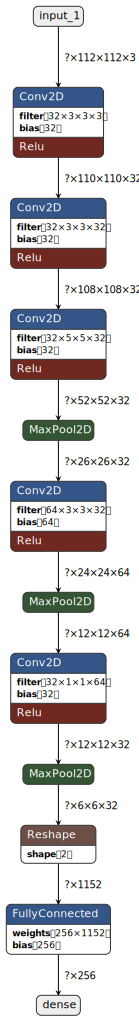
\includegraphics[scale=0.25]{Imagens/rafael_student_r8g8b8_tflite}
	\end{center}
	\caption {Arquitetura do modelo Rafael-2} \legend {Fonte: Autor}
\end{figure}
%
% \begin{center}
% \begin{table}[htb]
% \centering
% \ABNTEXfontereduzida
% \caption[Acurácia dos modelos]{Acurácia dos modelos.}
% \begin{tabular}{ |c|c|c|c| }
% 	% Fonte: https://www.seeedstudio.com/blog/2019/10/24/microcontrollers-for-machine-learning-and-ai/
% 	\hline
% 	\textbf{CPU (Clock Speed)} 	& \textbf{RAM}  & \textbf{Preço} & \textbf{Link} \\
% 	\hline
% 	Quad-core Cortex-A53 (2.30GHz)	& 1GB		& \$129.99	 & https://www.seeedstudio.com/Coral-Dev-Board-p-2900.html \\
% 	Quad-core ARM A57 (1.43GHz) 	& 4GB		& \$89.00	 & https://www.seeedstudio.com/NVIDIAr-Jetson-Nanotm-Developer-Kit-p-2916.html \\
% 	RISC-V Dual Core (400Mhz)  	& 8MB		& \$40.90	 & https://www.seeedstudio.com/Sipeed-MAix-GO-Suit-for-RISC-V-AI-IoT-p-2874.html \\
% 	Cortex-A72 - ARM v8 (1.5GHz)	& 1GB 		& \$35.90	 & https://www.seeedstudio.com/Raspberry-Pi-4-Computer-Model-B-1GB-p-4078.html \\
%
% 	\hline
% \end{tabular}
% \legend{Fonte: Autor}
% \end{table}
% \end{center}
%
% % % ---
% % \chapter{Morbi ultrices rutrum lorem.}
% % % ---
% % \lipsum[30]
% %
% % % ---
% % \chapter{Cras non urna sed feugiat cum sociis natoque penatibus et magnis dis
% % parturient montes nascetur ridiculus mus}
% % % ---
% %
% % \lipsum[31]
% %
% % % ---
% % \chapter{Fusce facilisis lacinia dui}
% % % ---
% %
% % \lipsum[32]
%
%
\end{anexosenv}


\end{document}
